% Created 2021-09-27 Mon 12:01
% Intended LaTeX compiler: xelatex
\documentclass[letterpaper]{article}
\usepackage{graphicx}
\usepackage{grffile}
\usepackage{longtable}
\usepackage{wrapfig}
\usepackage{rotating}
\usepackage[normalem]{ulem}
\usepackage{amsmath}
\usepackage{textcomp}
\usepackage{amssymb}
\usepackage{capt-of}
\usepackage{hyperref}
\setlength{\parindent}{0pt}
\usepackage[margin=1in]{geometry}
\usepackage{fontspec}
\usepackage{svg}
\usepackage{cancel}
\usepackage{indentfirst}
\setmainfont[ItalicFont = LiberationSans-Italic, BoldFont = LiberationSans-Bold, BoldItalicFont = LiberationSans-BoldItalic]{LiberationSans}
\newfontfamily\NHLight[ItalicFont = LiberationSansNarrow-Italic, BoldFont       = LiberationSansNarrow-Bold, BoldItalicFont = LiberationSansNarrow-BoldItalic]{LiberationSansNarrow}
\newcommand\textrmlf[1]{{\NHLight#1}}
\newcommand\textitlf[1]{{\NHLight\itshape#1}}
\let\textbflf\textrm
\newcommand\textulf[1]{{\NHLight\bfseries#1}}
\newcommand\textuitlf[1]{{\NHLight\bfseries\itshape#1}}
\usepackage{fancyhdr}
\pagestyle{fancy}
\usepackage{titlesec}
\usepackage{titling}
\makeatletter
\lhead{\textbf{\@title}}
\makeatother
\rhead{\textrmlf{Compiled} \today}
\lfoot{\theauthor\ \textbullet \ \textbf{2021-2022}}
\cfoot{}
\rfoot{\textrmlf{Page} \thepage}
\renewcommand{\tableofcontents}{}
\titleformat{\section} {\Large} {\textrmlf{\thesection} {|}} {0.3em} {\textbf}
\titleformat{\subsection} {\large} {\textrmlf{\thesubsection} {|}} {0.2em} {\textbf}
\titleformat{\subsubsection} {\large} {\textrmlf{\thesubsubsection} {|}} {0.1em} {\textbf}
\setlength{\parskip}{0.45em}
\renewcommand\maketitle{}
\author{Exr0n}
\date{\today}
\title{Rubisco}
\hypersetup{
 pdfauthor={Exr0n},
 pdftitle={Rubisco},
 pdfkeywords={},
 pdfsubject={},
 pdfcreator={Emacs 28.0.50 (Org mode 9.4.4)}, 
 pdflang={English}}
\begin{document}

\tableofcontents

\#ref \#disorganized

\section{Overview}
\label{sec:org32019e1}
\begin{itemize}
\item Rubisco is apparently a cool protein
\item Most abundant protein in the world
\item Enzyme that is very slow, which is why plants make so much of it
\item Rubisco in \href{https://pdb101.rcsb.org/motm/11}{pop science}
\end{itemize}

\section{Slide Intro}
\label{sec:org7ef0ca1}
\begin{figure}[htbp]
\centering
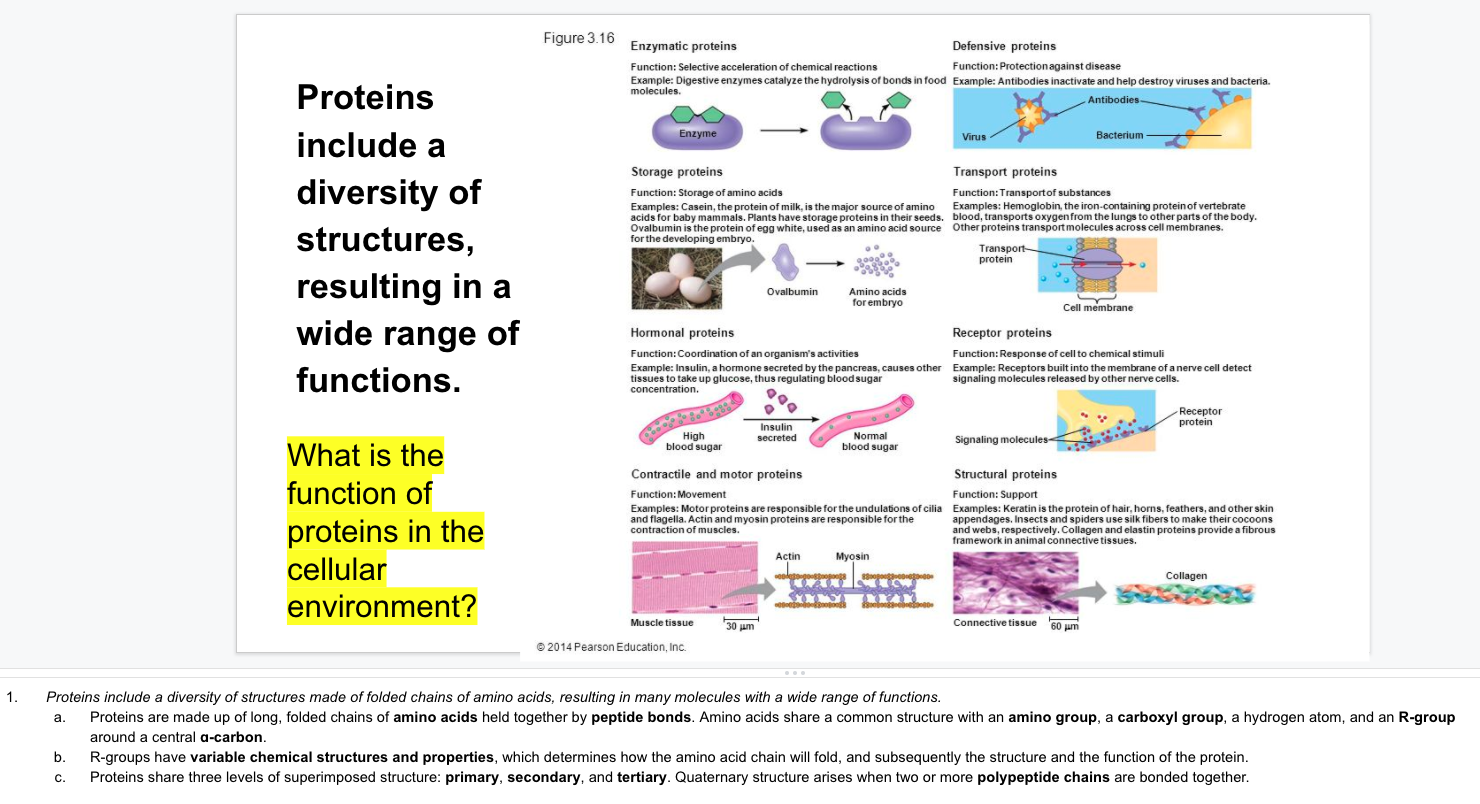
\includegraphics[width=.9\linewidth]{./20200924144612.png}
\caption{Pasted image}
\end{figure}

\section{Carbon Fixation}
\label{sec:org2e229c5}
\begin{itemize}
\item Turning carbon from the air into carbohydrates
\item Combines carbon from \(CO_2\), light, and water to get carbohydrates

\begin{itemize}
\item \(6CO_2 + 6H_2O + light = \text{carbs}\) \# Faults
\end{itemize}

\item Rubisco sometimes accidentally binds oxygen to a sugar chain in a
process called photorespiration

\begin{itemize}
\item The cell actually has to expend more energy to fix this mistake
\end{itemize}

\item Also it's like really really slow, processing around 3 reactions per
second instead of other enzymes which often process thousands
\end{itemize}

\href{Pasted image 20200929151124.png.org}{Pasted image
20200929151124.png}

\noindent\rule{\textwidth}{0.5pt}
\end{document}
